% Compile from docs/ with latexmk -pdf final_project_report.tex or Tectonic.
\documentclass[conference,letterpaper]{IEEEtran}
\usepackage[T1]{fontenc}
\usepackage{mathptmx,graphicx,cite,booktabs,tabularx,balance}
\usepackage[hidelinks]{hyperref}
\graphicspath{{figures/}}
\urlstyle{same}
\newcolumntype{Y}{>{\raggedright\arraybackslash}X}
\hypersetup{pdftitle={Design and Verification of a Single-Cycle Processor for a Ten-Instruction RV32I Subset},pdfauthor={Ankit Raj Singh, Rashmi Anand, Ayush, Saumya, and Samiksha Jangid}}
\begin{document}
\title{Design and Verification of a Single-Cycle Processor for a Ten-Instruction RV32I Subset}
\author{\IEEEauthorblockN{Ankit Raj Singh, Rashmi Anand, Ayush, Saumya, and Samiksha Jangid}
\IEEEauthorblockA{Department of CSE (AI)\\Newton School of Technology, Sonipat}}
\maketitle
\thispagestyle{plain}\pagestyle{plain}
\begin{abstract}
This work presents a 32-bit single-cycle Verilog processor for ten RV32I instructions spanning arithmetic, word transfers, and conditional control flow. A mixed assembly program sums three integers, stores six at byte address 64, and reloads that value into a register. Cycle-level traces identify the two taken backward branches and the edges that commit the store and load. All eleven simulation suites passed. A processor-level acceptance bench compared the program counter, 32 registers, and every word of its 32-word test RAM after each of 23 instruction steps. A controlled modification to the instruction decoder triggered a failure at the expected instruction. Generic synthesis reported 22,445 cells. The load datapath is a candidate for the cycle-time limit; the assumed gate-delay model gives an illustrative 70--140 MHz range. Device-level characterization remains open.
\end{abstract}
\begin{IEEEkeywords}
RISC-V, single-cycle processor, Verilog, instruction decoding, functional verification, logic synthesis
\end{IEEEkeywords}
\section{Introduction}
Correct arithmetic alone does not establish that a processor executes programs correctly. A store can issue the right data at the wrong address, a load can write back the address instead of the returned data, or a branch can skip the instruction that consumes a result. These interactions motivate observing a value from its creation in the arithmetic logic unit (ALU) through memory and subsequent control flow.

The project implements a teaching subset of RV32I~\cite{isa}. The supported instructions are ADD, SUB, AND, OR, XOR, ADDI, LW, SW, BEQ, and BNE. Phase~1 established sequential fetch and register arithmetic. Phase~2 integrated memory access and conditional next-PC selection, tested the completed processor, and evaluated its hardware cost. The evaluation asks whether a mixed program produces the predicted state at each relevant edge, whether the regression detects an erroneous decoder enable, and what the generic mapping establishes about timing and resource use. The design and recorded evidence are available in the repository~\cite{project}.

\subsection{Design Requirements and Evidence}
The processor must support three observable classes of change: a value written to a register, a value written to data memory, and a change to the address of the next instruction. Instructions often exercise more than one class. A load reads a register to calculate an address, obtains data from memory, and writes it into a second register. A branch consumes two register values and changes the PC while preserving both values. The verification plan uses the expected state at the clock boundary as the common contract across these instruction classes.

The report proceeds from this contract to its implementation and measured behavior. Appendix~\ref{app:baseline} shows the arithmetic baseline. The full datapath and instruction encodings appear in Appendix~\ref{app:enc}. Appendices~\ref{app:memory} and~\ref{app:assembly} trace memory and branches. Appendix~\ref{app:accept} isolates a decoder fault; Appendix~\ref{app:repro} explains how to reproduce the measurements. An address such as \texttt{0x40} is hexadecimal. In the examples that address is decimal 64 and refers to word 16 of a 32-bit memory. The data stored at that address depends on the program.

\section{Literature Review}
The RV32I base instruction set defines a 32-bit load/store architecture with fixed-width base instructions, 32 integer registers, and immediate encodings that keep register fields in consistent positions~\cite{isa}. These choices simplify a teaching datapath because the same register-file ports serve arithmetic, memory-address, and branch-comparison operations. Patterson and Hennessy present the single-cycle organization as a direct mapping from instruction semantics to fetch, decode, execute, memory, and writeback hardware~\cite{cod}. Harris and Harris use the same progression to show how a working single-cycle datapath can be divided first into multi-cycle steps and then into pipeline stages~\cite{harris}.

The three organizations make different timing and control trade-offs. A single-cycle processor completes every instruction in one long clock period, so its CPI is one and its clock is constrained by the slowest instruction, normally a load. A multi-cycle processor reuses hardware across shorter cycles under finite-state control, reducing the clock period while giving different instructions different cycle counts. A pipelined processor overlaps instructions and can approach one completed instruction per cycle after filling, but it requires forwarding, stalls, and branch recovery. The course project specification identifies the single-cycle processor as the functional baseline from which a five-stage implementation and hazard handling can later be studied.

Open-source RISC-V cores demonstrate additional design points. PicoRV32 is a configurable, size-oriented core that implements a wider RV32I/RV32IMC scope and uses a multi-cycle organization to reduce hardware cost~\cite{picorv32}. NERV is explicitly described as an educational RISC-V processor and is used as a simple target for formal ISA checking~\cite{nerv}. These cores pursue flexibility, compactness, or formal compliance. The present work instead fixes a ten-instruction subset and exposes the complete datapath so that instruction fields, control signals, and clock-edge state changes can be explained directly.

Processor verification also ranges from directed simulation to formal proof. Directed self-checking programs are effective for demonstrating a concrete path through arithmetic, memory, and branches, and waveforms help localize an incorrect enable or selection. The riscv-formal framework defines the RISC-V Formal Interface and generates bounded checks for architectural behavior~\cite{riscvformal}. This project uses directed simulation because the submitted core does not expose RVFI and because the required deliverables emphasize programs and waveform evidence. The whole-state acceptance bench reduces a common weakness of directed testing by comparing every register and test-memory word after each executed instruction. Formal compliance across all encodings remains future work.

\section{Proposed Solution}
\subsection{Processor Architecture}

The core follows the single-cycle organization described in~\cite{cod}. Between successive rising edges, the current program counter (PC) selects an instruction, the register file supplies operands, and combinational logic determines the next PC and any pending writes. The rising edge commits the state changes. The instruction following a load can read the new register value during the next cycle.

The default organization contains 64 instruction words, 32 register locations, and 256 data words. Separate instruction and data memories permit instruction fetch during a load or store. Synchronous reset selects PC zero and suppresses writes to registers and data RAM. Register x0 always reads as zero and discards writes. The completion flag in the top-level wrapper detects repeated PC samples at a terminal self-branch. The core continues executing the branch.

\subsection{Datapath and Instruction Decode}

Table~\ref{tab:modules} identifies the twelve blocks integrated into the core. Fig.~\ref{fig:load_path} illustrates two selections made during a load. The ALU input multiplexer selects the sign-extended offset to form the address. The writeback multiplexer subsequently selects the RAM output for the destination register.

\begin{figure}[t]\centering
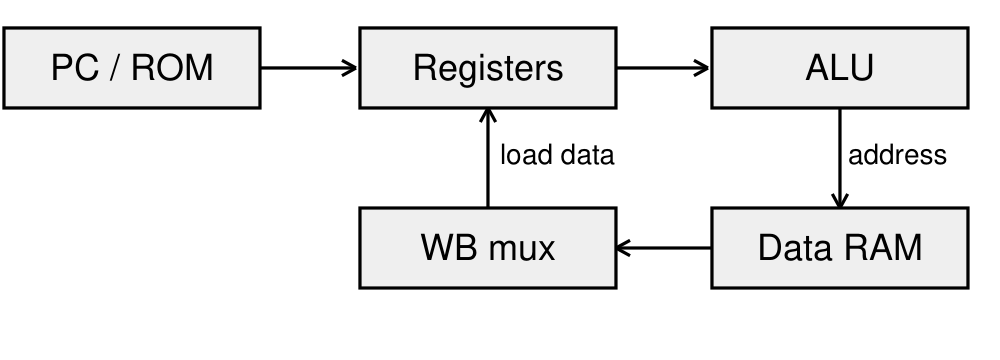
\includegraphics[width=\columnwidth]{final_load_path.png}
\caption{Load data path. The base register and signed offset form the byte address. The selected RAM word returns to the register file for the rising-edge write.}\label{fig:load_path}\end{figure}

\begin{table}[t]\centering\footnotesize
\caption{Integrated RTL Modules}\label{tab:modules}
\setlength{\tabcolsep}{3pt}
\begin{tabularx}{\columnwidth}{@{}lY@{}}\toprule
RTL module & Role in the integrated datapath\\\midrule
program\_counter & Commits next PC at the rising edge. Synchronous reset selects address zero.\\
instruction\_memory & Byte-addressed combinational fetch from the initialized word image.\\
control\_unit & Validates opcode and function bits and drives the control truth table.\\
register\_file & Two asynchronous reads and one rising-edge write. x0 reads zero.\\
immediate\_generator & Reassembles and sign-extends I, S and B immediates.\\
alu\_src\_mux / alu\_control & Select register or immediate operand B and decode the ALU operation.\\
alu & Performs 32-bit arithmetic and logic. Subtraction supplies branch equality.\\
data\_memory & Asynchronous word reads and synchronous writes with range and alignment checks.\\
writeback\_mux & Selects ALU result or load data for the destination register.\\
branch\_target / next\_pc\_mux & Add B-offset to the current PC and select target or PC + 4.\\
\bottomrule\end{tabularx}\end{table}

A program is loaded as hexadecimal instruction words. The decoder reads selected bit positions to decide which registers to read and which parts of the CPU may write a result.

At PC zero, instruction memory supplies 0x00300093, which encodes ADDI x1, x0, 3. The 12-bit immediate holds three, the first source register field selects x0, and the destination field selects x1. The function bits are 000 and the opcode is 0010011. The ALU adds zero and three, x1 captures three, and the PC advances by four bytes.

Later, ADDI x1, x1, -1 decrements the loop counter. Its immediate field contains twelve one bits. Sign extension copies the leading one into the upper twenty bits, giving 0xffffffff. Adding that 32-bit pattern to 3 yields 2.

Table~\ref{tab:decode} lists the main decoder outputs. The six control bits, from left to right, denote RegWrite, ALUSrc, MemRead, MemWrite, ResultSrc, and Branch. For LW, the ALU calculates the effective address and the memory supplies the writeback value. For SW, RAM captures the second source register at the addressed word.

\begin{table}[t]\centering\footnotesize
\caption{Main Decoder Truth Table}\label{tab:decode}
\setlength{\tabcolsep}{3pt}
\begin{tabularx}{\columnwidth}{@{}lYlllll@{}}\toprule
Op. & Opcode & $f_3$ & $f_7$ & Controls & ALU & Imm\\\midrule
ADD & 0110011 & 000 & 0000000 & 100000 & 10 & 11\\
SUB & 0110011 & 000 & 0100000 & 100000 & 10 & 11\\
AND & 0110011 & 111 & 0000000 & 100000 & 10 & 11\\
OR & 0110011 & 110 & 0000000 & 100000 & 10 & 11\\
XOR & 0110011 & 100 & 0000000 & 100000 & 10 & 11\\
ADDI & 0010011 & 000 & - & 110000 & 00 & 00\\
LW & 0000011 & 010 & - & 111010 & 00 & 00\\
SW & 0100011 & 010 & - & 010100 & 00 & 01\\
BEQ & 1100011 & 000 & - & 000001 & 01 & 10\\
BNE & 1100011 & 001 & - & 000001 & 01 & 10\\
Default & other & - & - & 000000 & 11 & 11\\
\bottomrule\end{tabularx}\end{table}

ALUOp 00 selects addition, 01 subtraction, 10 R-type decoding and 11 the default operation. ImmSrc 00 selects I, 01 selects S, 10 selects B and 11 yields zero.

BEQ selects the target when subtraction yields zero. BNE selects it when subtraction yields a nonzero result. An unsupported encoding leaves register and memory writes disabled and advances the PC by four.

\subsection{PC Selection and Effective Addresses}
With fixed-width 32-bit instructions, the sequential successor is four bytes beyond the current PC. The branch target and the sequential successor are computed concurrently. The decoder must first assert Branch. BEQ then selects the target when the ALU zero flag is high; BNE selects it when the flag is low. In either fall-through case the CPU selects PC + 4.
The current PC, rather than the sequential successor, is the base for the target. This choice matters in a backward loop. With the branch at address 20 and a displacement of $-8$, using 24 as the base would land at 16 and omit the addition at 12. Checking only that the PC moved backward would miss this error.

The effective data address is $R[rs1]+\mathrm{signext}(offset)$. Word alignment requires the two low address bits to be zero. The RAM index drops those two bits after validating the address range. At depth 256 the last valid aligned byte address is 1020. Simply truncating a larger address would risk writing a valid low-numbered word. The storage bench tests both the rejected access and the previously stored data to detect such aliasing.

\subsection{Write Enables, Reset, and Completion}
The main decoder chooses which state elements may change. The integrated core gates the register and memory write enables with reset. Resetting a running program therefore restarts instruction fetch and prevents a pending write during reset. The arrays retain their contents across that reset; their deterministic initial zeros arise from the simulation models. This distinction matters when rerunning a workload in the same simulation.

The completion detector belongs to the wrapper. An ordinary instruction that writes x0 can still advance the PC, and a loop through several different addresses continues to advance and redirect it. A terminal BEQ comparing x0 with itself and using a displacement of zero repeatedly selects the same PC. Observing repeated samples gives the bench a convenient completion indication without adding a halt instruction to the processor ISA.

\section{Verification Method}

The regression compiles the Verilog benches with Icarus Verilog 13.0 and runs the simulations with VVP~\cite{icarus}. Module tests isolate control, storage, arithmetic, and selection behavior. Integrated programs exercise the interfaces between blocks. The branch suite observes both the selected next PC before the clock edge and the committed PC after it. A separate processor acceptance bench specifies the expected state transitions directly for its program, independently of the RTL decoder.

\subsection{Cycle-Level State Comparison}

The acceptance bench drives a 10 ns clock, holds synchronous reset for two rising edges, and releases it on a falling edge. After each instruction it compares the new PC, all 32 registers, and the complete 32-word test RAM with expected state. Sampling after nonblocking updates settle avoids comparing a new prediction with the preceding register contents. A four-state comparison flags unexpected unknown values.

For example, the store at PC 0x08 executes with x1 equal to 64 and x2 equal to -7. The expected changes are a write of -7 to RAM word 16 and a PC update to 0x0c. Every register and all other memory words must retain their previous values. The next instruction must then load -7 into x3. Checking all locations reveals an unintended second write even when the intended destination contains the correct value.

Subsequent ALU instructions produce -14, 0, -7, 64, and 0 in x4 through x8. A taken branch skips a store to byte address 68 and another branch skips a write of 99 to x9. Each control-flow decision therefore has an observable consequence for subsequent program state.

\subsection{Failure Criteria and Controlled Fault}

The regression driver collects one log per suite, checks process status, detects explicit failure messages, and requires completion markers. The final condition matters because some earlier benches can finish normally after reporting a failed comparison. A suite failure produces a nonzero aggregate exit status while the remaining suites still run.

To test the failure path, a disposable RTL copy widened the ADDI decoder to accept the unsupported ORI function. The test image, expected states, and runner were held constant. This experiment examines whether a known fault can be localized to its first erroneous control decision.

\section{Results and Discussion}

\subsection{Arithmetic and Memory Operations}

For operands 10 and 20, the integration test observed 30 for ADD, 10 for 20 minus 10, zero for AND, and 30 for both OR and XOR. These operands share no set bit, so OR and XOR coincide for this input. In the mixed program, XOR of two copies of six produces zero. A subsequent branch consumes that result.

The integrated ALU suite checks 0x7fffffff + 1. The hardware returns 0x80000000. The destination retains the low 32 bits. Their signed interpretation is the most negative 32-bit value. The same suite checks subtraction across the opposite boundary.

The memory workload first establishes a known nonzero value. ADDI sets x1 to 64 and x2 to 25. SW places 25 at byte address 64, LW reloads it into x3, and ADD produces 50 in x4. This sequence exercises the path from a register into RAM and back into arithmetic without preloading the expected RAM value.

The assembly program uses byte addresses. The Verilog RAM holds 32-bit words. Bytes 64 through 67 belong to word 16, so an aligned word access translates to index 64 / 4 = 16. An offset of +8 from the same base selects word 18; an offset of -4 selects word 15.

Varying the address detects indexing faults which a repeated access to one word can miss. In this design a misaligned or out-of-range read returns zero and an invalid store leaves memory unchanged.

\subsection{Mixed Assembly Program}

The mixed program initializes x1 to three, x2 to zero, and x3 to 64. ADD at PC 0x0c adds the counter to the accumulator. ADDI at 0x10 decrements the counter, and BNE at 0x14 branches backward while the updated value differs from zero. The target is the branch PC plus a signed displacement of -8 bytes. Table~\ref{tab:loop} gives the observed PC selections. The counter and accumulator values follow from the executed instructions.

\begin{table}[t]\centering\footnotesize
\caption{Three Visits to the Branch at PC 0x14}\label{tab:loop}
\setlength{\tabcolsep}{3pt}
\begin{tabularx}{\columnwidth}{@{}lccYl@{}}\toprule
Time (ns) & Counter & Sum & Decision & Next PC\\\midrule
71 & 2 & 3 & Taken & 0x0c\\
101 & 1 & 5 & Taken & 0x0c\\
131 & 0 & 6 & Fall through & 0x18\\
\bottomrule\end{tabularx}\end{table}

When the counter reaches zero, control falls through to the store at 0x18. Fig.~\ref{fig:mixed_trace} shows the associated memory enables. At 141 ns the processor presents byte address 64 and store data six. The rising edge at 145 ns commits six to RAM word 16. The load then selects the same address, presents six for writeback at 151 ns, and commits the value to x4 at 155 ns.

\begin{figure}[t]\centering
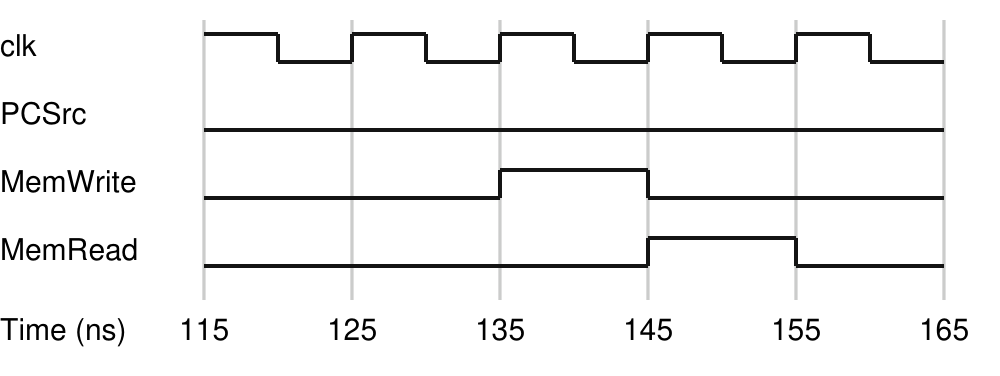
\includegraphics[width=\columnwidth]{final_mixed_trace.png}
\caption{Mixed-program waveform from 115 to 165 ns. MemWrite is asserted during the store, followed by MemRead during the load. The rising edges at 145 and 155 ns commit the RAM and register writes, respectively.}\label{fig:mixed_trace}\end{figure}

Later the program compares x8 with zero at PC 0x30. XOR has produced zero, so BEQ jumps to 0x3c. That skips both an ADDI and a store. The test checks the skipped register x9 and the data word at byte address 68; both stay zero.

The program reaches its terminal branch at PC 0x54 with x11 equal to 42. Across all six branch programs, BEQ was taken nine times and fell through four times. BNE was taken seven times and fell through five times. These counts exclude terminal self-branches. For a taken branch with displacement +4, the target equals the sequential address. The bench checks the branch-select signal explicitly to distinguish those outcomes.

\subsection{Unsupported Instructions and Fault Detection}

At PCs 0x3c through 0x54, the acceptance program presents MUL, SLL, ORI, LB, SB, BLT, and an unrecognized opcode. Each advances the PC by four, preserves register and RAM contents, and leaves register write, memory read, memory write, and branch selection inactive. A legal load afterward returns -7 to x10. An attempted write to x0 leaves it zero. These observations characterize the project policy for the tested encodings.

The modified decoder encountered instruction 0x0010e493 at PC 0x44, the encoding for ORI x9, x1, 1. The acceptance bench detected the forbidden register-write enable before the wrong value could commit. Both the standalone decoder suite and the complete-processor suite failed, yielding nine passing suites, two failing suites, and a nonzero exit status. Restoring the submitted design gave the eleven passing suites in Table~\ref{tab:regression}.

\begin{table}[t]\centering\footnotesize
\caption{Directed Regression Results}\label{tab:regression}
\setlength{\tabcolsep}{3pt}
\begin{tabularx}{\columnwidth}{@{}lY@{}}\toprule
Suite & Passing observations\\\midrule
fetch & Three benches passed. PC reset and update, instruction ROM, integrated fetch.\\
storage & Both benches passed. Register reads/writes, x0, data RAM enables and bounds.\\
mux\_immediate & Five benches passed. Immediate generation (17 cases), ALU source (10), writeback (10), next PC (11), branch target (18).\\
alu & Two benches passed. 17 ALU cases and 14 ALU-control cases.\\
phase1 & Three benches passed. Decoder (20 cases), arithmetic core and one-word memory boundaries.\\
full\_cpu & Passed. Earlier complete-core regression retained for compatibility.\\
integration & 20 checks passed. All ten supported instructions, both branch outcomes, register and RAM results.\\
memory & 34 checks passed. Loads, stores, offsets, read after write, multiple locations and skipped memory operations.\\
alu\_integration & 63 checks passed. ALU controls/results, wraparound, signed limits, addresses and branch comparison.\\
branch & Six assembly programs passed. All ten instructions in the mixed program, forward/backward offsets and exact PC routes.\\
final\_cpu & 23 retirements passed. Cycle-by-cycle architectural state, unsupported instructions, recovery and x0 protection.\\
\bottomrule\end{tabularx}\end{table}

\subsection{Coverage Interpretation}
The module tests and program tests answer different diagnostic questions. An ALU test can isolate an incorrect truth function by driving overlapping bit patterns. An integration test adds instruction decode, register selection, write enable, and the edge that commits the result. A passing module test alongside a failing integration case therefore directs attention toward wiring, control, or clocking. It does not by itself identify which of those interfaces is responsible.

The six assembly workloads check 92 executed steps and perform 955 comparisons. The comparison count includes route, control, and end-state observations. The 23 steps of the separate acceptance program each include a complete register and memory comparison. Adding these numbers would mix test assertions, instructions, and test configurations. Results are reported with their own units throughout.

The seven unsupported words target different parts of decode, including a known opcode with an unsupported function and an entirely unrecognized opcode. The experiments establish the behavior of those examples. Formal properties over all possible words, broader generated program coverage, and physical implementation tests would answer additional questions beyond the directed regression.

\section{Hardware Cost and Timing}

The committed synthesis report records passing Verilator lint and Yosys structural checks~\cite{project,yosys}. Generic mapping produced 22,445 cells, including 9,543 multiplexers, 9,216 enabled flip-flops, and 32 resettable flip-flops for the program counter. The storage counts follow directly from the array dimensions: $256\times32=8{,}192$ data-memory bits and $32\times32=1{,}024$ register-file bits. Asynchronous reads also require selection logic to route one of many words to the output.

LW spans instruction ROM, decode, register read, address addition, asynchronous data RAM read, writeback selection and register setup. The load therefore combines two storage reads with arithmetic on one clock path. Branches traverse register reads, subtraction, comparison and next-PC selection.

The ALU has a longest generic path of 69 logic levels. The branch-target adder has 62. These are separately mapped block depths. A device clock rating requires a target library, constraints and routed timing. The 10 ns simulation clock exercises functional behavior.

\subsection{First-Order Timing Estimate}
The project's analytical model sums generic block depths along the data portion of the load path: 10 levels for register read, one for operand selection, 69 for the ALU, nine for RAM read, and one for writeback. This gives about 90 levels. It combines individually mapped block maxima and an assumed mux depth. It does not measure an actual end-to-end path through an integrated, placed design. Instruction fetch, clock-to-output delay, register setup, routing and fanout would also enter a physical timing budget.

Assuming 0.08, 0.12, or 0.16 ns per level gives nominal delays of 7.2, 10.8, or 14.4 ns, respectively. The reciprocals are approximately 139, 93, and 69 MHz. The rounded 70--140 MHz interval expresses sensitivity to an assumption. It is distinct from both the 10 ns simulation stimulus and the device-specific result that an FPGA or ASIC timing tool would report. Mapping the RAM to a synchronous block memory, for example, could require an extra load cycle and a change to the interface.

\subsection{Comparison with Alternative Organizations}
For $N$ executed instructions the ideal single-cycle execution time is $NT_\mathrm{single}$. The design has one instruction in flight and one cycle per instruction. Its long load path therefore constrains the clock used for short logical operations as well. This organization makes a waveform straightforward to interpret: the PC at a particular edge identifies the single instruction whose effects are being committed.

A multi-cycle version could keep intermediate values between fetch, decode, execute, memory and writeback. A controller would select the required steps for each instruction. A shorter clock period could then be traded against multiple cycles per instruction. A pipelined version could overlap those stages across instructions. A load immediately followed by an ADD using its result would require forwarding or a stall, and a taken branch would require handling younger instructions fetched on the sequential path. Neither alternative was implemented or benchmarked in this project. The comparison identifies the design changes needed to obtain a different throughput or timing target.

\section{Individual Contributions}

Ankit Raj Singh integrated the core and top-level datapath. Rashmi Anand integrated and verified load/store execution. Ayush verified integrated ALU behavior and documented synthesis and timing. Samiksha Jangid developed the branch and assembly workloads. Saumya integrated the regression, developed the processor-level acceptance test, and prepared the verification and final submission materials.

The role exchange for Phase~2 is reflected in this breakdown: Samiksha completed the M13 branch, PC-route, and assembly workload originally allocated to Saumya, while Saumya completed the M14 full-processor regression and M16 documentation work originally allocated to Samiksha. The final demonstration remains a team deliverable.

\section{Reproducibility}

From the repository root, \texttt{./run\_tests.sh} compiles and runs all eleven suites with Bash, Icarus Verilog, and VVP. The archived evidence includes 17 logs, six instruction traces in CSV format, and 26 VCD waveforms~\cite{project}. The CSV and waveform records for the mixed program support Table~\ref{tab:loop} and Fig.~\ref{fig:mixed_trace}. The annotated acceptance program and self-checking bench specify the expected state comparisons. The resource counts and logic depths come from the separately recorded synthesis run.

\subsection{Inspection of the Recorded Evidence}
The submitted records permit three independent checks of the mixed workload. The CSV file records one sample per executed step. Filtering on PC 0x14 yields the three next-PC choices in Table~\ref{tab:loop}. The VCD file records changes between those samples, including the edge that writes RAM word 16. Finally, the branch testbench compares the complete expected register and memory arrays after the workload. Together these checks distinguish selecting the right address, asserting the right enable, and committing the right data.

For the acceptance program, Table~\ref{tab:acceptance} groups the checks by their expected architectural effect. The image contains 25 instruction words. Two words on skipped paths are never executed, and the test stops after the first execution of the terminal self-branch, giving 23 checked steps. This workload uses a different image from the mixed program in Fig.~\ref{fig:mixed_trace}; each PC in the table refers to the acceptance image.

\begin{table}[t]\centering\footnotesize
\caption{Processor-Level Acceptance Record}\label{tab:acceptance}
\begin{tabularx}{\columnwidth}{@{}lY@{}}\toprule
PC or range (hex) & Expected and observed effect\\\midrule
00--0c & Establish base 64 and data $-7$, store to word 16, and load $-7$ into x3.\\
10--20 & ADD, SUB, AND, OR, and XOR produce $-14$, 0, $-7$, 64, and 0.\\
24--38 & BEQ skips the store at 28. BNE falls through at 2c and redirects at 34, leaving x9 equal to one.\\
3c--54 & Seven unsupported encodings each advance the PC by four with no register or RAM changes.\\
58--60 & LW reloads $-7$ into x10. A write targeting x0 is discarded. The self-branch holds PC at 60.\\\bottomrule
\end{tabularx}\end{table}

\section{Limitations and Conclusion}

The integrated core executed the ten supported instructions across arithmetic, memory transfer, and conditional control flow. The mixed program provides a traceable chain from the backward branch through RAM to the final register write. Independent state comparisons and a controlled decoder fault demonstrated that the regression can detect a specific unintended write request at its source. These results establish directed coverage for the tested programs and encodings. Exhaustive verification and device-specific frequency characterization remain open.

\begin{thebibliography}{9}
\bibitem{isa} A. Waterman and K. Asanovi\'c, Eds., \emph{The RISC-V Instruction Set Manual, Volume I: Unprivileged ISA}, ver. 20191213, Dec. 2019, ch. 2.
\bibitem{project} Project team, \emph{Single-Cycle RISC-V Processor: RTL, Verification Evidence, and Synthesis Results}, project repository, Nov. 2026. [Online]. Available: \url{https://github.com/roboayushh/RISC-V}
\bibitem{cod} D. A. Patterson and J. L. Hennessy, \emph{Computer Organization and Design RISC-V Edition: The Hardware/Software Interface}, 2nd ed. Morgan Kaufmann, 2020, ch. 4.
\bibitem{harris} S. L. Harris and D. M. Harris, \emph{Digital Design and Computer Architecture: RISC-V Edition}. Morgan Kaufmann, 2021, ch. 7.
\bibitem{picorv32} YosysHQ, ``PicoRV32---A size-optimized RISC-V CPU,'' GitHub repository. [Online]. Available: \url{https://github.com/YosysHQ/picorv32}
\bibitem{nerv} YosysHQ, ``NERV---Naive Educational RISC-V Processor,'' GitHub repository. [Online]. Available: \url{https://github.com/YosysHQ/nerv}
\bibitem{riscvformal} YosysHQ, ``RISC-V Formal Verification Framework,'' GitHub repository. [Online]. Available: \url{https://github.com/YosysHQ/riscv-formal}
\bibitem{icarus} S. Williams, \emph{Icarus Verilog}, ver. 13.0. [Online]. Available: \url{https://github.com/steveicarus/iverilog}
\bibitem{yosys} C. Wolf, \emph{Yosys Open SYnthesis Suite}. [Online]. Available: \url{https://yosyshq.readthedocs.io/}
\end{thebibliography}
% Full-width experimental records accompany the two-column paper.
\clearpage\onecolumn
\appendices
\section{Phase 1 Baseline and Integration Contracts}
\label{app:baseline}
The first milestone established an observable arithmetic core before adding branch and memory execution. Its 14-step program exercises six instructions and checks register writeback at the active edge. Table~\ref{tab:baseline} gives the opening sequence. The constants 10 and 20 deliberately occupy different bit positions. Their AND is zero, and their OR and XOR both equal 30. Later vectors use overlapping operands to separate the two logical functions.

\begin{table}[!ht]\centering
\caption{Opening Instructions of the Phase 1 Arithmetic Program}\label{tab:baseline}
\begin{tabularx}{.96\linewidth}{@{}lllY@{}}\toprule
PC & Instruction & Result & Observable change\\\midrule
0x00 & \texttt{addi x1,x0,10} & x1 = 10 & Decode immediate addition and enable destination write.\\
0x04 & \texttt{addi x2,x0,20} & x2 = 20 & A second register retains its own value.\\
0x08 & \texttt{add x3,x1,x2} & x3 = 30 & Read both preceding results in the same cycle.\\
0x0c & \texttt{sub x4,x2,x1} & x4 = 10 & Operand order matters for subtraction.\\
0x10 & \texttt{and x5,x1,x2} & x5 = 0 & The two input words have no shared set bits.\\
0x14 & \texttt{or x6,x1,x2} & x6 = 30 & Either set input bit produces a set output bit.\\
0x18 & \texttt{xor x7,x1,x2} & x7 = 30 & Differing input bits produce a set output bit.\\\bottomrule
\end{tabularx}\end{table}

\begin{figure}[!ht]\centering
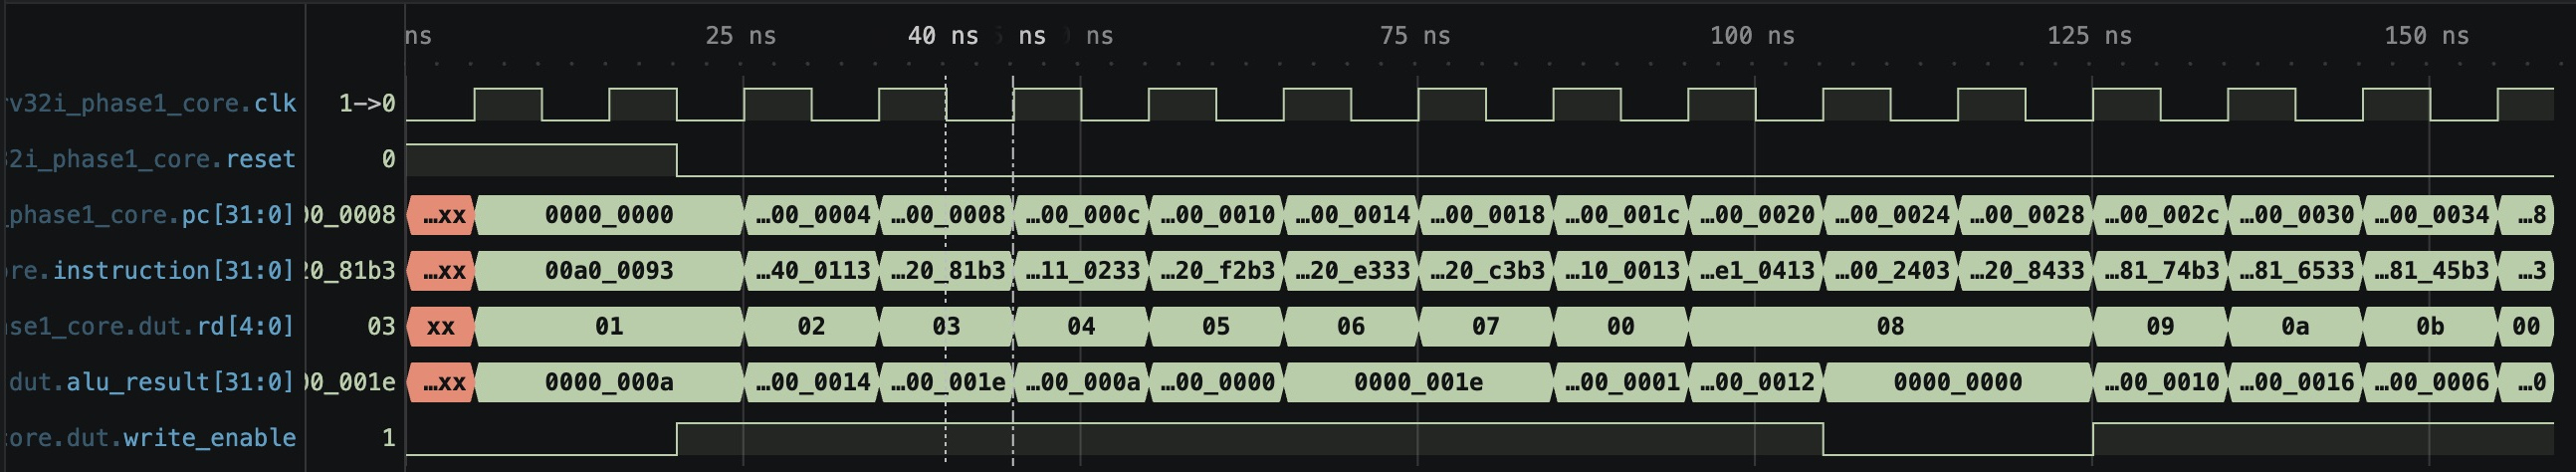
\includegraphics[width=.96\linewidth,height=.24\textheight,keepaspectratio]{waveforms/tb_rv32i_phase1_core.jpg}
\caption{Phase 1 arithmetic waveform. The ADD at PC 0x08 presents destination x3 and result 0x1e at 40 ns. The rising edge at 45 ns commits the write. Subsequent PC and operand changes belong to SUB.}
\end{figure}

\subsection{What changes when memory and branches are connected?}
A passing ADD establishes the register-to-ALU-to-register path. Phase 2 introduces a second writeback source, an independently enabled RAM write port, and a second source of PC updates. A useful integration test must therefore separate an ALU result from a RAM word and a branch target from the sequential PC. The load/store example uses address 64 and value 25; a mux that selected the address would produce an immediately distinguishable value in x3. The branch example skips a store and checks that the destination word retains its initial value.

\subsection{Reset and fetch boundaries}
Instruction fetch uses byte addresses with four-byte alignment. For example, PC 0x08 selects ROM word two. The ROM model returns the canonical \texttt{ADDI x0,x0,0} for a misaligned or out-of-range fetch. Executing this word leaves x0 unchanged and advances the PC. This behavior differs from the deliberate terminal self-branch. The depth-one test separately covers the case in which address zero is the sole valid word. A memory implementation that assumes a nonzero address index width needs a special case for this configuration.

\clearpage
\section{Instruction Encoding and Datapath Derivations}\label{app:enc}
\subsection{From the instruction word to its operands}
The instruction format determines which bits name registers and which contribute to a signed constant. Source register indices occupy bits 19--15 and 24--20 when present. Bits 11--7 identify the destination in register-writing instructions and contribute immediate bits in stores and branches. Table~\ref{tab:fields} shows the implemented immediate construction. Here $I[i:j]$ denotes a slice of the 32-bit instruction word.

\begin{table}[!ht]\centering
\caption{Immediate Fields Reassembled by the Implemented Decoder}\label{tab:fields}
\begin{tabularx}{.96\linewidth}{@{}llY@{}}\toprule
Format & Source fields, high to low & Use in the datapath\\\midrule
I & $I[31:20]$ & Sign-extend the 12-bit value for ADDI or a load address.\\
S & $I[31:25],I[11:7]$ & Concatenate the two fields, sign-extend, and add to the base for SW.\\
B & $I[31],I[7],I[30:25],I[11:8],0$ & Form a signed byte displacement and add it to the branch PC.\\
Default & Zero & Drive a defined immediate for unused selector values.\\\bottomrule
\end{tabularx}\end{table}

\subsection{Three words from the mixed program}
\textbf{Immediate arithmetic.} At PC 0x10, word \texttt{fff08093} encodes \texttt{addi x1,x1,-1}. Its high 12 bits are all ones. Replicating the sign bit produces 0xffffffff. On the first iteration the ALU input from x1 is three. The low 32 bits of the sum are two, which are committed back into x1. Zero-extension would instead add 4095, and the loop would follow the wrong sequence of counter values even if branch decoding were correct.

\textbf{Backward branch.} At PC 0x14, word \texttt{fe009ce3} encodes \texttt{bne x1,x0,loop}. The extracted byte displacement is 0xfffffff8 ($-8$). The branch-target adder therefore offers 0x0c on every visit. The target value is available even on the final iteration. The comparison decides whether the mux selects it: subtracting zero from a nonzero x1 yields a clear zero flag; subtracting zero from zero sets it. On this final visit the target remains 0x0c but the selected next PC is 0x18.

\textbf{Store and load.} The successive words \texttt{0021a023} and \texttt{0001a203} encode \texttt{sw x2,0(x3)} and \texttt{lw x4,0(x3)}. Both add a zero offset to base 64. During the store, x2 supplies six and the RAM write enable controls the rising-edge update. During the load, RAM read data goes through the writeback mux into x4. The equal addresses and different destinations explain why the ALU result alone cannot establish that both instructions executed correctly.

\begin{figure}[!ht]\centering
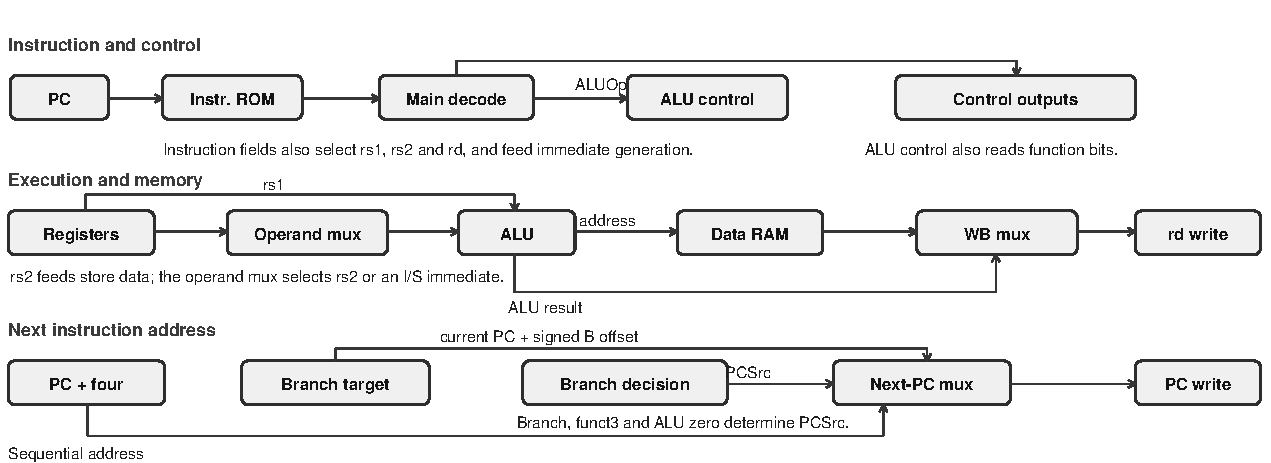
\includegraphics[width=.86\linewidth]{final_core_datapath.pdf}
\caption{Integrated signal paths, grouped by function. Register reads and decode proceed in parallel. The WB mux returns the selected ALU or RAM value to the destination register. The next-PC mux selects the sequential or branch address. All three groups operate within the same instruction cycle.}
\label{fig:complete-core}\end{figure}

\subsection{Branch limits and unused encodings}
B-immediates encode even byte displacements. This design fetches four-byte instructions, so the boundary program uses the largest positive displacement compatible with that alignment, $+4092$, and the minimum signed displacement, $-4096$. A BEQ at 0x0004 lands at 0x1000. A later BNE at 0x1004 returns to 0x0004. The image uses 1,028 ROM words because the addresses are far apart, although just nine instruction steps are checked. ROM footprint, distance jumped, and dynamic instruction count measure different properties.

\clearpage
\section{Memory Transactions and Waveform Interpretation}\label{app:memory}
The memory workload starts with x1 = 64 and x2 = 25. Its purpose is to follow a known value through both directions of the memory interface and then consume it as an operand. The memory holds complete 32-bit words. Byte address 0x40 corresponds to word index 16. In the waveform, 0x19 denotes decimal 25 and 0x32 denotes decimal 50.

\begin{figure}[!ht]\centering
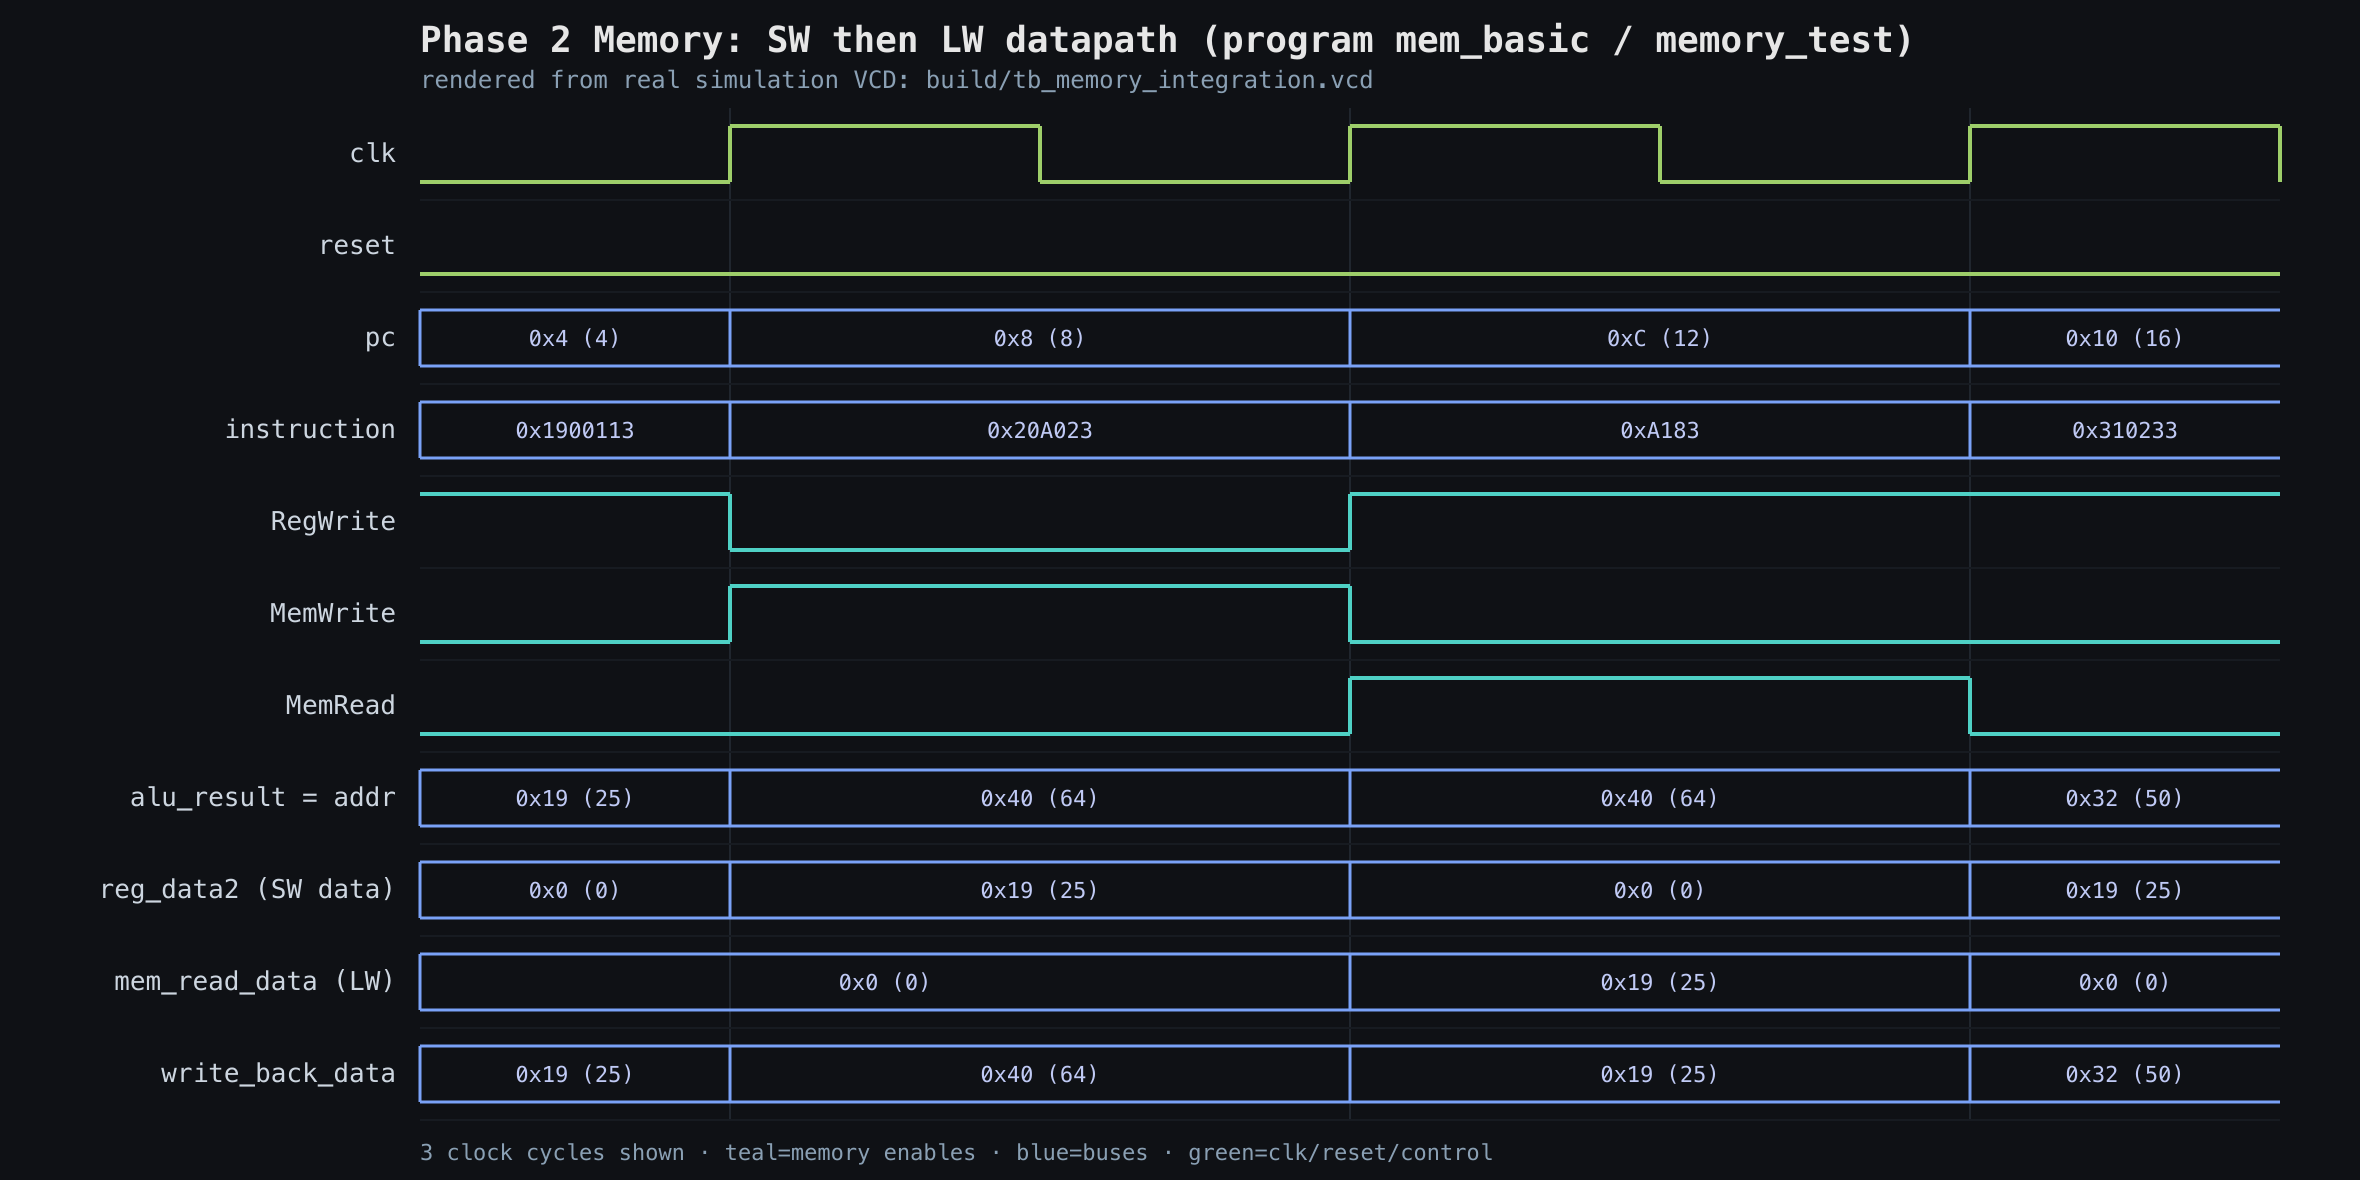
\includegraphics[width=.96\linewidth,height=.29\textheight,keepaspectratio]{waveforms/mem_sw_lw_zoom.png}
\caption{Recorded memory integration simulation for the value 25. The store at PC 0x08 drives an effective address of 0x40. The load at PC 0x0c selects the same address and routes 0x19 back to the register file. The following ADD consumes the loaded word.}
\end{figure}

\begin{table}[!ht]\centering
\caption{Observable Differences Between the Three Adjacent Instructions}
\begin{tabularx}{.96\linewidth}{@{}lccY@{}}\toprule
Instruction & Memory read & Memory write & Edge outcome\\\midrule
SW x2,0(x1) & 0 & 1 & RAM word 16 receives 25. No destination register is written.\\
LW x3,0(x1) & 1 & 0 & Register x3 captures the selected RAM word, 25.\\
ADD x4,x2,x3 & 0 & 0 & The ALU adds 25 and 25. Register x4 captures 50.\\\bottomrule
\end{tabularx}\end{table}

\subsection{Address, enable, and data are independent observations}
The same numerical address appears in both memory cycles. A correct address with a missing write enable would leave the previous RAM contents intact. A correct read with a wrong writeback selection would place 64 in x3. An implementation that updated the register file during SW could corrupt an unrelated value even if the RAM word were correct. The integration suite checks register and memory outcomes, while the waveform identifies which interface to inspect first when an outcome differs.

\subsection{Boundary and interference cases}
The storage suite checks aligned words at byte addresses 0, 4, 8, 64, and 1020. A disabled read returns zero. The misaligned address 0x42 and the out-of-range address 0x1000 also yield zero in the tested configuration. A subsequent read of 0x40 checks the previously stored 25. Other programs check writing zero over a location, loading 0xffffffff at positive and negative offsets, and preserving memory across a skipped store. These cases exercise address validation, enable gating, and the distinction between a legitimate zero value and a failed transaction.

\clearpage
\section{Assembly Workloads and Instruction Trace}\label{app:assembly}
The six assembly workloads use RV32I instructions with compressed instructions and linker relaxation disabled. The image builder assembles and links text at address zero, extracts the text section, and converts each group of four little-endian bytes into one hexadecimal word for the ROM. For example, bytes \texttt{93 00 30 00} become \texttt{00300093}. GNU disassembly is retained under the build directory for examining encodings. The regression consumes committed images directly.

\begin{table}[!ht]\centering
\caption{Coverage and Outcomes of the Six Directed Programs}
\begin{tabularx}{.98\linewidth}{@{}lrrrY@{}}\toprule
Program & ROM words & Steps & Checks & Selected result\\\midrule
Arithmetic & 15 & 15 & 137 & AND, OR and XOR of 12 and 10 give 8, 14 and 6.\\
Memory & 11 & 11 & 121 & Addresses 64 and 68 hold 25 and 50.\\
Branch equal & 16 & 18 & 194 & A taken BEQ skips x3 and the loop terminates.\\
Branch not equal & 13 & 15 & 167 & Unequal initial operands take BNE.\\
Mixed integration & 22 & 24 & 203 & All ten instruction types execute; x4 = 6 and x11 = 42.\\
Offset boundaries & 1,028 & 9 & 133 & Forward and backward aligned boundary targets are reached.\\\midrule
Total & & 92 & 955 & 25 functional branch decisions, excluding terminal branches.\\\bottomrule
\end{tabularx}\end{table}

\subsection{The portion of the mixed trace after the loop}
The CSV records a sample before the state update. Thus a time in Table~\ref{tab:tail} identifies the instruction whose effects will commit on the next rising edge. The route proceeds directly from 0x30 to 0x3c, and later from 0x48 to 0x54. Those gaps are successful control-flow observations. The absence of writes on the skipped paths is checked independently in the final state.

\begin{table}[!ht]\centering\small
\caption{Mixed Program After Its Final Backward-Branch Decision}\label{tab:tail}
\begin{tabularx}{.98\linewidth}{@{}rlllY@{}}\toprule
Time (ns) & PC & Next PC & Instruction & Expected effect\\\midrule
131 & 14 & 18 & BNE & Counter zero. Fall through to the store.\\
141 & 18 & 1c & SW & Store the sum at byte address 64.\\
151 & 1c & 20 & LW & Load six into x4.\\
161 & 20 & 24 & SUB & x5 receives $6-6=0$.\\
171 & 24 & 28 & AND & x6 receives $6\mathbin{\&}6=6$.\\
181 & 28 & 2c & OR & x7 receives six OR zero, giving six.\\
191 & 2c & 30 & XOR & x8 receives six XOR six, giving zero.\\
201 & 30 & 3c & BEQ & Zero equals x0. Skip x9 write and store.\\
211 & 3c & 40 & ADDI & Set x10 to one as a success marker.\\
221 & 40 & 44 & BNE & Loaded and accumulated values agree. Fall through.\\
231 & 44 & 48 & ADDI & Set x11 to 42.\\
241 & 48 & 54 & BEQ & Skip the remaining failure path.\\
251 & 54 & 54 & BEQ & Observe the terminal self-branch.\\\bottomrule
\end{tabularx}\end{table}

A trace row includes a candidate branch target even for arithmetic instructions, because the adder continuously computes its output. The selected next PC and PCSrc identify whether that candidate has any architectural effect. Reading the target bus alone can therefore give a misleading interpretation of sequential instructions.

\clearpage
\section{Processor Acceptance and Fault Localization}\label{app:accept}
The final testbench isolates seven unsupported encodings in a contiguous part of its instruction image. Before this sequence, x9 holds one and RAM word 16 holds $-7$. The expected outcome at every step is sequential PC progression with the register file and memory intact. Fig.~\ref{fig:unsupported} shows the actual core signals recorded during the passing run. PC and instruction are hexadecimal buses.

\begin{figure}[!ht]\centering
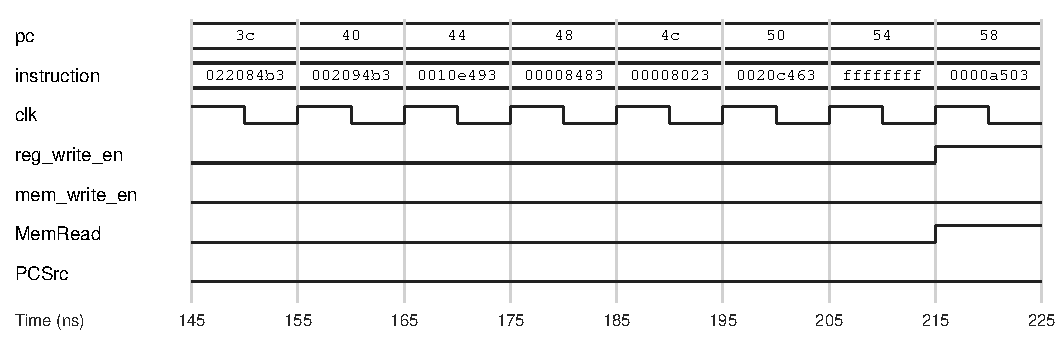
\includegraphics[width=.96\linewidth]{final_unsupported_trace.pdf}
\caption{Acceptance-test VCD excerpt rendered from the integrated core. The seven words at PCs 0x3c through 0x54 keep the write enables, MemRead, and PCSrc low. At PC 0x58, a legal load reasserts MemRead and register write enable.}\label{fig:unsupported}
\end{figure}

\begin{table}[!ht]\centering\small
\caption{Negative Test Vectors and Decode Boundaries}
\begin{tabularx}{.98\linewidth}{@{}lllY@{}}\toprule
PC & Word & Encoding & Fault class probed\\\midrule
3c & 022084b3 & MUL & R-type function extension outside supported arithmetic.\\
40 & 002094b3 & SLL & Unsupported R-type shift function.\\
44 & 0010e493 & ORI & Immediate arithmetic opcode with unsupported function.\\
48 & 00008483 & LB & Load opcode with byte-width function.\\
4c & 00008023 & SB & Store opcode with byte-width function.\\
50 & 0020c463 & BLT & Branch opcode with unsupported relational comparison.\\
54 & ffffffff & Unknown & Unsupported primary opcode.\\\bottomrule
\end{tabularx}\end{table}

\subsection{Why the injected ORI defect fails at 0x44}
The injected decoder accepts the ORI function in the ADDI path. The expected write enable for this word is zero. When the modified decoder asserts it, the bench can identify the erroneous control signal before waiting for a destination value. In the passing design the following legal LW at 0x58 reads the sentinel word into x10, providing a positive check immediately after seven negative ones. The paired observations distinguish suppression of an individual encoding from a core stuck with all enables low.

\subsection{Independent expectations and diagnostics}
The bench maintains an expected register array and expected RAM array. Before the store it changes just the predicted RAM word; before a register-producing instruction it changes just the intended register. After the edge it identifies the first mismatching index, expected value and observed value. This is a different observation from comparing the decoder outputs. A decoder could generate the right enables while a downstream mux selects the wrong value. Conversely, an enabled write of an already stored value could leave the final array unchanged. The control checks and state comparisons cover both cases within this directed program.

\clearpage
\section{Reproduction and Interpretation of Measurements}\label{app:repro}
\subsection{Simulation and image verification}
Run the following commands from the repository root. The simulation uses Bash, Icarus Verilog and VVP. The optional image check additionally requires GNU RISC-V Binutils and Python 3. The archived evidence can be inspected without rebuilding the images.
\begin{verbatim}
./run_tests.sh
cat build/regression/final_cpu.log
cat build/branch/integration.csv
bash scripts/build_branch_programs.sh --check
\end{verbatim}
The aggregate command produces a suite name, PASS or FAIL, and a final count. Each suite's individual output remains in \texttt{build/regression/}. A compilation error, a simulator failure, or an absent completion marker causes the driver to report a failed suite. During source-level debugging, the per-suite log identifies the first useful diagnostic. The CSV identifies the executing PC. The VCD then exposes the corresponding combinational controls and the edge that commits their effect.

\subsection{Interpreting the synthesis outputs}
The command \texttt{./synthesize.sh} lints the wrapper with Verilator, executes the ALU integration simulation, synthesizes the core with Yosys, runs structural checks, and writes a netlist. It also synthesizes selected modules independently for topological path analysis. The raw report is \texttt{synthesis\_report.txt}; the generated netlist is \texttt{netlist/rv32i\_core\_netlist.v}. Rebuilding this flow refreshes both tracked artifacts. The counts below refer to the committed generic mapping.

\begin{table}[!ht]\centering
\caption{Generic Implementation Evidence and Its Interpretation}
\begin{tabularx}{.98\linewidth}{@{}llY@{}}\toprule
Quantity & Value & Interpretation\\\midrule
Hierarchy cells & 22,445 & Total mapped cells across the processor hierarchy.\\
RAM flip-flops & 8,192 & 256 data words, 32 bits per word.\\
Register-file flip-flops & 1,024 & 32 words, 32 bits per word in the generic storage mapping.\\
PC flip-flops & 32 & Resettable registered instruction address.\\
Multiplexers & 9,543 & Includes selection logic associated with asynchronous reads.\\
ALU / branch-target depth & 69 / 62 & Longest paths of separately synthesized blocks, in generic levels.\\
Assumed load-path sum & About 90 levels & Includes the ALU maximum, RAM and register reads, and two selectors.\\\bottomrule
\end{tabularx}\end{table}

\subsection{What each timing number can establish}
The simulation clock is an input selected by the testbench. The logic-depth results count generic levels. The estimates of approximately 139, 93, and 69 MHz follow only after assuming a delay per level. None of these observations identifies the worst endpoint in a physically routed device. A target-specific experiment needs a selected device or standard-cell library, clock and I/O constraints, mapped storage, and a timing report after implementation. That report would identify startpoint, endpoint, data arrival time, required time and slack.

The principal design trade-off follows directly from the load sequence. Register read, effective-address generation, asynchronous memory read, and writeback all occur between the same two active edges. Replacing that RAM with synchronous block RAM changes when the data becomes available. A corresponding multi-cycle controller or pipeline boundary would be a microarchitectural change requiring new load-use and branch tests, even if the assembly program and its final answer remain the same.

\end{document}
